\PassOptionsToPackage{unicode=true}{hyperref} % options for packages loaded elsewhere
\PassOptionsToPackage{hyphens}{url}
%
\documentclass[]{article}
\usepackage{lmodern}
\usepackage{amssymb,amsmath}
\usepackage{ifxetex,ifluatex}
\usepackage{fixltx2e} % provides \textsubscript
\ifnum 0\ifxetex 1\fi\ifluatex 1\fi=0 % if pdftex
  \usepackage[T1]{fontenc}
  \usepackage[utf8]{inputenc}
  \usepackage{textcomp} % provides euro and other symbols
\else % if luatex or xelatex
  \usepackage{unicode-math}
  \defaultfontfeatures{Ligatures=TeX,Scale=MatchLowercase}
\fi
% use upquote if available, for straight quotes in verbatim environments
\IfFileExists{upquote.sty}{\usepackage{upquote}}{}
% use microtype if available
\IfFileExists{microtype.sty}{%
\usepackage[]{microtype}
\UseMicrotypeSet[protrusion]{basicmath} % disable protrusion for tt fonts
}{}
\IfFileExists{parskip.sty}{%
\usepackage{parskip}
}{% else
\setlength{\parindent}{0pt}
\setlength{\parskip}{6pt plus 2pt minus 1pt}
}
\usepackage{hyperref}
\hypersetup{
            pdftitle={homework},
            pdfauthor={tetero},
            pdfborder={0 0 0},
            breaklinks=true}
\urlstyle{same}  % don't use monospace font for urls
\usepackage[margin=1in]{geometry}
\usepackage{color}
\usepackage{fancyvrb}
\newcommand{\VerbBar}{|}
\newcommand{\VERB}{\Verb[commandchars=\\\{\}]}
\DefineVerbatimEnvironment{Highlighting}{Verbatim}{commandchars=\\\{\}}
% Add ',fontsize=\small' for more characters per line
\usepackage{framed}
\definecolor{shadecolor}{RGB}{248,248,248}
\newenvironment{Shaded}{\begin{snugshade}}{\end{snugshade}}
\newcommand{\AlertTok}[1]{\textcolor[rgb]{0.94,0.16,0.16}{#1}}
\newcommand{\AnnotationTok}[1]{\textcolor[rgb]{0.56,0.35,0.01}{\textbf{\textit{#1}}}}
\newcommand{\AttributeTok}[1]{\textcolor[rgb]{0.77,0.63,0.00}{#1}}
\newcommand{\BaseNTok}[1]{\textcolor[rgb]{0.00,0.00,0.81}{#1}}
\newcommand{\BuiltInTok}[1]{#1}
\newcommand{\CharTok}[1]{\textcolor[rgb]{0.31,0.60,0.02}{#1}}
\newcommand{\CommentTok}[1]{\textcolor[rgb]{0.56,0.35,0.01}{\textit{#1}}}
\newcommand{\CommentVarTok}[1]{\textcolor[rgb]{0.56,0.35,0.01}{\textbf{\textit{#1}}}}
\newcommand{\ConstantTok}[1]{\textcolor[rgb]{0.00,0.00,0.00}{#1}}
\newcommand{\ControlFlowTok}[1]{\textcolor[rgb]{0.13,0.29,0.53}{\textbf{#1}}}
\newcommand{\DataTypeTok}[1]{\textcolor[rgb]{0.13,0.29,0.53}{#1}}
\newcommand{\DecValTok}[1]{\textcolor[rgb]{0.00,0.00,0.81}{#1}}
\newcommand{\DocumentationTok}[1]{\textcolor[rgb]{0.56,0.35,0.01}{\textbf{\textit{#1}}}}
\newcommand{\ErrorTok}[1]{\textcolor[rgb]{0.64,0.00,0.00}{\textbf{#1}}}
\newcommand{\ExtensionTok}[1]{#1}
\newcommand{\FloatTok}[1]{\textcolor[rgb]{0.00,0.00,0.81}{#1}}
\newcommand{\FunctionTok}[1]{\textcolor[rgb]{0.00,0.00,0.00}{#1}}
\newcommand{\ImportTok}[1]{#1}
\newcommand{\InformationTok}[1]{\textcolor[rgb]{0.56,0.35,0.01}{\textbf{\textit{#1}}}}
\newcommand{\KeywordTok}[1]{\textcolor[rgb]{0.13,0.29,0.53}{\textbf{#1}}}
\newcommand{\NormalTok}[1]{#1}
\newcommand{\OperatorTok}[1]{\textcolor[rgb]{0.81,0.36,0.00}{\textbf{#1}}}
\newcommand{\OtherTok}[1]{\textcolor[rgb]{0.56,0.35,0.01}{#1}}
\newcommand{\PreprocessorTok}[1]{\textcolor[rgb]{0.56,0.35,0.01}{\textit{#1}}}
\newcommand{\RegionMarkerTok}[1]{#1}
\newcommand{\SpecialCharTok}[1]{\textcolor[rgb]{0.00,0.00,0.00}{#1}}
\newcommand{\SpecialStringTok}[1]{\textcolor[rgb]{0.31,0.60,0.02}{#1}}
\newcommand{\StringTok}[1]{\textcolor[rgb]{0.31,0.60,0.02}{#1}}
\newcommand{\VariableTok}[1]{\textcolor[rgb]{0.00,0.00,0.00}{#1}}
\newcommand{\VerbatimStringTok}[1]{\textcolor[rgb]{0.31,0.60,0.02}{#1}}
\newcommand{\WarningTok}[1]{\textcolor[rgb]{0.56,0.35,0.01}{\textbf{\textit{#1}}}}
\usepackage{graphicx,grffile}
\makeatletter
\def\maxwidth{\ifdim\Gin@nat@width>\linewidth\linewidth\else\Gin@nat@width\fi}
\def\maxheight{\ifdim\Gin@nat@height>\textheight\textheight\else\Gin@nat@height\fi}
\makeatother
% Scale images if necessary, so that they will not overflow the page
% margins by default, and it is still possible to overwrite the defaults
% using explicit options in \includegraphics[width, height, ...]{}
\setkeys{Gin}{width=\maxwidth,height=\maxheight,keepaspectratio}
\setlength{\emergencystretch}{3em}  % prevent overfull lines
\providecommand{\tightlist}{%
  \setlength{\itemsep}{0pt}\setlength{\parskip}{0pt}}
\setcounter{secnumdepth}{0}
% Redefines (sub)paragraphs to behave more like sections
\ifx\paragraph\undefined\else
\let\oldparagraph\paragraph
\renewcommand{\paragraph}[1]{\oldparagraph{#1}\mbox{}}
\fi
\ifx\subparagraph\undefined\else
\let\oldsubparagraph\subparagraph
\renewcommand{\subparagraph}[1]{\oldsubparagraph{#1}\mbox{}}
\fi

% set default figure placement to htbp
\makeatletter
\def\fps@figure{htbp}
\makeatother


\title{homework}
\author{tetero}
\date{5/25/2020}

\begin{document}
\maketitle

\hypertarget{exercise-1-subsetting-and-statistics}{%
\subsection{Exercise 1 (Subsetting and
Statistics)}\label{exercise-1-subsetting-and-statistics}}

\textbf{(a)} Install and load the \texttt{ggplot2} package. \textbf{Do
not} include the installation command in your \texttt{.Rmd} file. (If
you do it will install the package every time you knit your file.)
\textbf{Do} include the command to load the package into your
environment.

\begin{Shaded}
\begin{Highlighting}[]
\KeywordTok{library}\NormalTok{(}\StringTok{"ggplot2"}\NormalTok{)}
\NormalTok{x =}\StringTok{ }\NormalTok{msleep}
\end{Highlighting}
\end{Shaded}

\textbf{(b)} Note that this dataset is technically a \texttt{tibble},
not a data frame. How many observations are in this dataset? How many
variables? What are the observations in this dataset?

It has 83 observations, 11 variables. The observations in this data set
are about mammals animals. It contains characteristics information about
sleep, awake, and body weights times. This data set in an expanded
collection of the mammals sleep dataset

\textbf{(c)} What is the mean hours of REM sleep of individuals in this
dataset?

\begin{Shaded}
\begin{Highlighting}[]
\KeywordTok{mean}\NormalTok{(x}\OperatorTok{$}\NormalTok{sleep_rem, }\DataTypeTok{na.rm =} \OtherTok{TRUE}\NormalTok{)}
\end{Highlighting}
\end{Shaded}

\begin{verbatim}
## [1] 1.87541
\end{verbatim}

\textbf{(d)} What is the standard deviation of brain weight of
individuals in this dataset?

\begin{Shaded}
\begin{Highlighting}[]
\KeywordTok{sd}\NormalTok{(x}\OperatorTok{$}\NormalTok{brainwt, }\DataTypeTok{na.rm =} \OtherTok{TRUE}\NormalTok{)}
\end{Highlighting}
\end{Shaded}

\begin{verbatim}
## [1] 0.9764137
\end{verbatim}

\textbf{(e)} Which observation (provide the \texttt{name}) in this
dataset gets the most REM sleep?

\begin{Shaded}
\begin{Highlighting}[]
\NormalTok{y =}\StringTok{ }\KeywordTok{max}\NormalTok{(x}\OperatorTok{$}\NormalTok{sleep_rem, }\DataTypeTok{na.rm =} \OtherTok{TRUE}\NormalTok{)}
\KeywordTok{subset}\NormalTok{(x}\OperatorTok{$}\NormalTok{name, x}\OperatorTok{$}\NormalTok{sleep_rem }\OperatorTok{==}\StringTok{ }\NormalTok{y)}
\end{Highlighting}
\end{Shaded}

\begin{verbatim}
## [1] "Thick-tailed opposum"
\end{verbatim}

\textbf{(f)} What is the average bodyweight of carnivores in this
dataset?

\begin{Shaded}
\begin{Highlighting}[]
\NormalTok{z =}\StringTok{ }\NormalTok{(}\KeywordTok{subset}\NormalTok{(x, x}\OperatorTok{$}\NormalTok{order }\OperatorTok{==}\StringTok{ "Carnivora"}\NormalTok{))}
\KeywordTok{mean}\NormalTok{(z}\OperatorTok{$}\NormalTok{bodywt)}
\end{Highlighting}
\end{Shaded}

\begin{verbatim}
## [1] 57.70525
\end{verbatim}

\begin{center}\rule{0.5\linewidth}{0.5pt}\end{center}

\hypertarget{exercise-2-plotting}{%
\subsection{Exercise 2 (Plotting)}\label{exercise-2-plotting}}

\textbf{(a)} Note that this dataset is a data frame and all of the
variables are numeric. How many observations are in this dataset? How
many variables? What are the observations in this dataset?

\begin{Shaded}
\begin{Highlighting}[]
\KeywordTok{library}\NormalTok{(MASS)}
\NormalTok{x2 =}\StringTok{ }\NormalTok{MASS}\OperatorTok{::}\NormalTok{birthwt}
\KeywordTok{str}\NormalTok{(x2)}
\end{Highlighting}
\end{Shaded}

\begin{verbatim}
## 'data.frame':    189 obs. of  10 variables:
##  $ low  : int  0 0 0 0 0 0 0 0 0 0 ...
##  $ age  : int  19 33 20 21 18 21 22 17 29 26 ...
##  $ lwt  : int  182 155 105 108 107 124 118 103 123 113 ...
##  $ race : int  2 3 1 1 1 3 1 3 1 1 ...
##  $ smoke: int  0 0 1 1 1 0 0 0 1 1 ...
##  $ ptl  : int  0 0 0 0 0 0 0 0 0 0 ...
##  $ ht   : int  0 0 0 0 0 0 0 0 0 0 ...
##  $ ui   : int  1 0 0 1 1 0 0 0 0 0 ...
##  $ ftv  : int  0 3 1 2 0 0 1 1 1 0 ...
##  $ bwt  : int  2523 2551 2557 2594 2600 2622 2637 2637 2663 2665 ...
\end{verbatim}

The birthwt dataset from the MASS package has data on 189 births at the
Baystate Medical Centre, Springfield, Massachusetts, during 1986. The
more important variables are low birth weight, a binary response
variable low. It is a data set of 189 observations and 10 variables.

\textbf{(b)} Create a scatter plot of birth weight (y-axis) vs mother's
weight before pregnancy (x-axis). Use a non-default color for the
points. (Also, be sure to give the plot a title and label the axes
appropriately.) Based on the scatter plot, does there seem to be a
relationship between the two variables? Briefly explain.

\begin{Shaded}
\begin{Highlighting}[]
\KeywordTok{plot}\NormalTok{(x2}\OperatorTok{$}\NormalTok{lwt, x2}\OperatorTok{$}\NormalTok{bwt, }\DataTypeTok{main =} \StringTok{"Birth weight vs mother’s weight before pregnancy"}\NormalTok{,}
     \DataTypeTok{xlab =} \StringTok{"Mother’s weight before pregnancy"}\NormalTok{, }\DataTypeTok{ylab =} \StringTok{"Birth weigh"}\NormalTok{, }\DataTypeTok{col =} \StringTok{"red"}\NormalTok{)}
\end{Highlighting}
\end{Shaded}

\begin{verbatim}
## Warning in title(...): conversion failure on 'Birth weight vs mother’s weight
## before pregnancy' in 'mbcsToSbcs': dot substituted for <e2>
\end{verbatim}

\begin{verbatim}
## Warning in title(...): conversion failure on 'Birth weight vs mother’s weight
## before pregnancy' in 'mbcsToSbcs': dot substituted for <80>
\end{verbatim}

\begin{verbatim}
## Warning in title(...): conversion failure on 'Birth weight vs mother’s weight
## before pregnancy' in 'mbcsToSbcs': dot substituted for <99>
\end{verbatim}

\begin{verbatim}
## Warning in title(...): conversion failure on 'Mother’s weight before pregnancy'
## in 'mbcsToSbcs': dot substituted for <e2>
\end{verbatim}

\begin{verbatim}
## Warning in title(...): conversion failure on 'Mother’s weight before pregnancy'
## in 'mbcsToSbcs': dot substituted for <80>
\end{verbatim}

\begin{verbatim}
## Warning in title(...): conversion failure on 'Mother’s weight before pregnancy'
## in 'mbcsToSbcs': dot substituted for <99>
\end{verbatim}

\begin{Shaded}
\begin{Highlighting}[]
\KeywordTok{abline}\NormalTok{(}\KeywordTok{lm}\NormalTok{(x2}\OperatorTok{$}\NormalTok{bwt }\OperatorTok{~}\StringTok{ }\NormalTok{x2}\OperatorTok{$}\NormalTok{lwt, }\DataTypeTok{data =}\NormalTok{ x2), }\DataTypeTok{col =} \StringTok{"blue"}\NormalTok{)}
\end{Highlighting}
\end{Shaded}

\includegraphics{w01-hw-oboffil2_files/figure-latex/unnamed-chunk-7-1.pdf}

It will say it is a weak correlation because the point doesn't show a
definite direction, and the regression line is almost horizontal.

\textbf{(c)} Create a scatter plot of birth weight (y-axis) vs mother's
age (x-axis). Use a non-default color for the points. (Also, be sure to
give the plot a title and label the axes appropriately.) Based on the
scatter plot, does there seem to be a relationship between the two
variables? Briefly explain.

\begin{Shaded}
\begin{Highlighting}[]
\KeywordTok{plot}\NormalTok{(x2}\OperatorTok{$}\NormalTok{age, x2}\OperatorTok{$}\NormalTok{bwt, }\DataTypeTok{main =} \StringTok{"Birth weight vs Mother’s age"}\NormalTok{,}
     \DataTypeTok{xlab =} \StringTok{"Mother’s age"}\NormalTok{, }\DataTypeTok{ylab =} \StringTok{"Birth weigh"}\NormalTok{, }\DataTypeTok{col =} \StringTok{"red"}\NormalTok{)}
\end{Highlighting}
\end{Shaded}

\begin{verbatim}
## Warning in title(...): conversion failure on 'Birth weight vs Mother’s age' in
## 'mbcsToSbcs': dot substituted for <e2>
\end{verbatim}

\begin{verbatim}
## Warning in title(...): conversion failure on 'Birth weight vs Mother’s age' in
## 'mbcsToSbcs': dot substituted for <80>
\end{verbatim}

\begin{verbatim}
## Warning in title(...): conversion failure on 'Birth weight vs Mother’s age' in
## 'mbcsToSbcs': dot substituted for <99>
\end{verbatim}

\begin{verbatim}
## Warning in title(...): conversion failure on 'Mother’s age' in 'mbcsToSbcs': dot
## substituted for <e2>
\end{verbatim}

\begin{verbatim}
## Warning in title(...): conversion failure on 'Mother’s age' in 'mbcsToSbcs': dot
## substituted for <80>
\end{verbatim}

\begin{verbatim}
## Warning in title(...): conversion failure on 'Mother’s age' in 'mbcsToSbcs': dot
## substituted for <99>
\end{verbatim}

\begin{Shaded}
\begin{Highlighting}[]
\KeywordTok{abline}\NormalTok{(}\KeywordTok{lm}\NormalTok{(x2}\OperatorTok{$}\NormalTok{bwt }\OperatorTok{~}\StringTok{ }\NormalTok{x2}\OperatorTok{$}\NormalTok{age, }\DataTypeTok{data =}\NormalTok{ x2), }\DataTypeTok{col =} \StringTok{"blue"}\NormalTok{)}
\end{Highlighting}
\end{Shaded}

\includegraphics{w01-hw-oboffil2_files/figure-latex/unnamed-chunk-8-1.pdf}

I will say it is not correlation because the point doesn't show a
specific direction and the regression line is almost horizontal

\textbf{(d)} Create side-by-side boxplots for birth weight grouped by
smoking status. Use non-default colors for the plot. (Also, be sure to
give the plot a title and label the axes appropriately.) Based on the
boxplot, does there seem to be a difference in birth weight for mothers
who smoked? Briefly explain.

\begin{Shaded}
\begin{Highlighting}[]
\KeywordTok{boxplot}\NormalTok{(x2}\OperatorTok{$}\NormalTok{bwt }\OperatorTok{~}\StringTok{ }\NormalTok{x2}\OperatorTok{$}\NormalTok{smoke, }\DataTypeTok{data =}\NormalTok{ x2, }\DataTypeTok{main =} \StringTok{"Birth weight grouped by smoking status"}\NormalTok{, }\DataTypeTok{xlab =} \StringTok{"Smoking Group"}\NormalTok{, }
        \DataTypeTok{ylab =} \StringTok{"Birth weight"}\NormalTok{, }\DataTypeTok{col =} \StringTok{"orange"}\NormalTok{,}
        \DataTypeTok{border =} \StringTok{"red"}\NormalTok{)  }
\end{Highlighting}
\end{Shaded}

\includegraphics{w01-hw-oboffil2_files/figure-latex/unnamed-chunk-9-1.pdf}

Yes, It looks like the average of women that smoke have a birth with the
lowest weight

\begin{center}\rule{0.5\linewidth}{0.5pt}\end{center}

\hypertarget{exercise-3-importing-data-more-plotting}{%
\subsection{Exercise 3 (Importing Data, More
Plotting)}\label{exercise-3-importing-data-more-plotting}}

\begin{Shaded}
\begin{Highlighting}[]
\KeywordTok{library}\NormalTok{(readr)}
\NormalTok{nutrition_}\DecValTok{2018}\NormalTok{ =}\StringTok{ }\KeywordTok{read_csv}\NormalTok{(}\StringTok{"nutrition-2018.csv"}\NormalTok{)}
\end{Highlighting}
\end{Shaded}

\begin{verbatim}
## Parsed with column specification:
## cols(
##   ID = col_character(),
##   Desc = col_character(),
##   Water = col_double(),
##   Calories = col_double(),
##   Protein = col_double(),
##   Fat = col_double(),
##   Carbs = col_double(),
##   Fiber = col_double(),
##   Sugar = col_double(),
##   Calcium = col_double(),
##   Potassium = col_double(),
##   Sodium = col_double(),
##   VitaminC = col_double(),
##   Chol = col_double(),
##   Portion = col_character()
## )
\end{verbatim}

\textbf{(a)} Create a histogram of \texttt{Calories}. Do not modify
\texttt{R}'s default bin selection. Make the plot presentable. Describe
the shape of the histogram. Do you notice anything unusual?

\begin{Shaded}
\begin{Highlighting}[]
\KeywordTok{hist}\NormalTok{(nutrition_}\DecValTok{2018}\OperatorTok{$}\NormalTok{Calories,}
     \DataTypeTok{xlab   =} \StringTok{"Calories per serving size"}\NormalTok{,}
     \DataTypeTok{main   =} \StringTok{"Histogram of Calories"}\NormalTok{,}
     \DataTypeTok{col    =} \StringTok{"blue"}\NormalTok{,}
     \DataTypeTok{border =} \StringTok{"red"}\NormalTok{)}
\end{Highlighting}
\end{Shaded}

\includegraphics{w01-hw-oboffil2_files/figure-latex/unnamed-chunk-11-1.pdf}

It is a right-skewed histogram, and we can see something unusual: food
that is close to 400 calories per serving and passing the 800 calories
per serving are frequent in the data set and disrupt the right shep of
the histogram

\textbf{(b)} Create a scatter plot of calories (y-axis) vs protein
(x-axis). Make the plot presentable. Do you notice any trends? Do you
think that knowing only the protein content of a food, you could make a
good prediction of the calories in the food?

\begin{Shaded}
\begin{Highlighting}[]
\KeywordTok{plot}\NormalTok{(nutrition_}\DecValTok{2018}\OperatorTok{$}\NormalTok{Calories }\OperatorTok{~}\StringTok{ }\NormalTok{nutrition_}\DecValTok{2018}\OperatorTok{$}\NormalTok{Protein, }\DataTypeTok{data =}\NormalTok{ nutrition_}\DecValTok{2018}\NormalTok{,}
     \DataTypeTok{xlab =} \StringTok{"Protein"}\NormalTok{,}
     \DataTypeTok{ylab =} \StringTok{"Calories"}\NormalTok{,}
     \DataTypeTok{main =} \StringTok{"calories vs Protein"}\NormalTok{,}
     \DataTypeTok{col  =} \StringTok{"red"}\NormalTok{,}
     \DataTypeTok{xlim=}\KeywordTok{c}\NormalTok{(}\DecValTok{0}\NormalTok{,}\DecValTok{80}\NormalTok{),}
     \DataTypeTok{ylim=}\KeywordTok{c}\NormalTok{(}\DecValTok{0}\NormalTok{,}\DecValTok{800}\NormalTok{))}
\KeywordTok{abline}\NormalTok{(}\KeywordTok{lm}\NormalTok{(nutrition_}\DecValTok{2018}\OperatorTok{$}\NormalTok{Calories }\OperatorTok{~}\StringTok{ }\NormalTok{nutrition_}\DecValTok{2018}\OperatorTok{$}\NormalTok{Protein, }\DataTypeTok{data =}\NormalTok{ nutrition_}\DecValTok{2018}\NormalTok{), }\DataTypeTok{col =} \StringTok{"blue"}\NormalTok{)}
\end{Highlighting}
\end{Shaded}

\includegraphics{w01-hw-oboffil2_files/figure-latex/unnamed-chunk-12-1.pdf}

We can see that a trend that shows that bigger the protein more calories
in the food, but we also find an essential portion of low protein with
high calories, even when we can try to predict the information, I don't
think it will be the best prediction

\textbf{(c)} Create a scatter plot of \texttt{Calories} (y-axis) vs
\texttt{4\ *\ Protein\ +\ 4\ *\ Carbs\ +\ 9\ *\ Fat} (x-axis). Make the
plot presentable. You will either need to add a new variable to the data
frame, or use the \texttt{I()} function in your formula in the call to
\texttt{plot()}. If you are at all familiar with nutrition, you may
realize that this formula calculates the calorie count based on the
protein, carbohydrate, and fat values. You'd expect then that the result
here is a straight line. Is it? If not, can you think of any reasons why
it is not?

\begin{Shaded}
\begin{Highlighting}[]
\NormalTok{Value =}\StringTok{ }\NormalTok{((}\DecValTok{4} \OperatorTok{*}\StringTok{ }\NormalTok{nutrition_}\DecValTok{2018}\OperatorTok{$}\NormalTok{Protein) }\OperatorTok{+}\StringTok{ }\NormalTok{(}\DecValTok{4} \OperatorTok{*}\StringTok{ }\NormalTok{nutrition_}\DecValTok{2018}\OperatorTok{$}\NormalTok{Carbs) }
         \OperatorTok{+}\StringTok{ }\NormalTok{(}\DecValTok{9} \OperatorTok{*}\StringTok{ }\NormalTok{nutrition_}\DecValTok{2018}\OperatorTok{$}\NormalTok{Fat))}

\KeywordTok{plot}\NormalTok{(nutrition_}\DecValTok{2018}\OperatorTok{$}\NormalTok{Calories }\OperatorTok{~}\StringTok{ }\NormalTok{Value, }\DataTypeTok{data =}\NormalTok{ nutrition_}\DecValTok{2018}\NormalTok{,}
     \DataTypeTok{xlab =} \StringTok{"Protein, Fat, Carbs times 4"}\NormalTok{,}
     \DataTypeTok{ylab =} \StringTok{"Calories"}\NormalTok{,}
     \DataTypeTok{main =} \StringTok{"Calories vs Protein, Fat and Carbs"}\NormalTok{,}
     \DataTypeTok{col  =} \StringTok{"red"}\NormalTok{)}
\KeywordTok{abline}\NormalTok{(}\KeywordTok{lm}\NormalTok{(nutrition_}\DecValTok{2018}\OperatorTok{$}\NormalTok{Calories }\OperatorTok{~}\StringTok{ }\NormalTok{Value, }\DataTypeTok{data =}\NormalTok{ nutrition_}\DecValTok{2018}\NormalTok{), }\DataTypeTok{col =} \StringTok{"blue"}\NormalTok{)}
\end{Highlighting}
\end{Shaded}

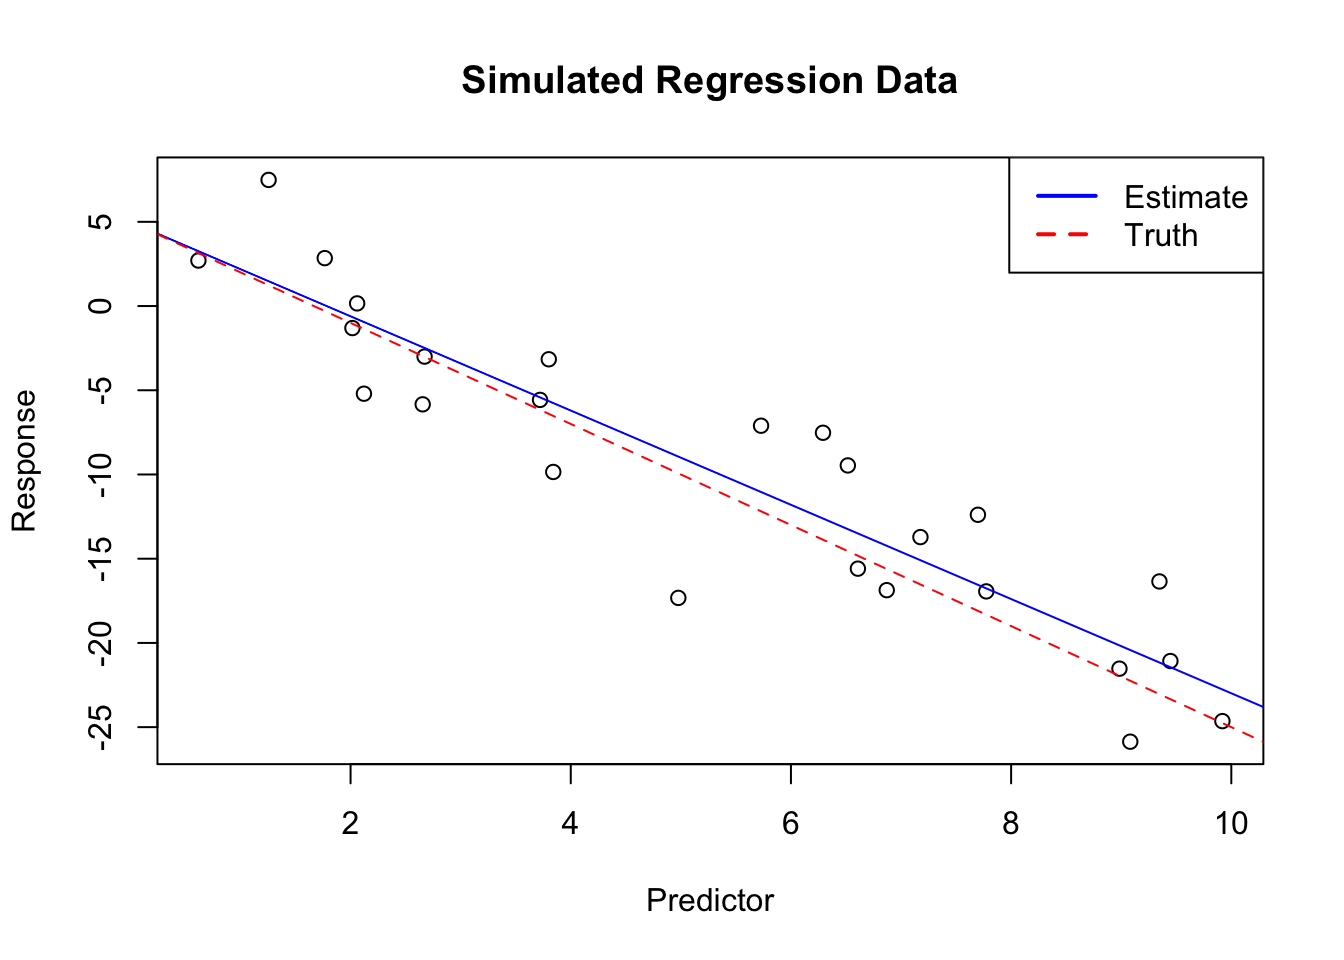
\includegraphics{w01-hw-oboffil2_files/figure-latex/unnamed-chunk-13-1.pdf}

It has a positive correlation, and it is almost a straight line, but you
can find that some food doesn't follow the trend of this especially the
food at 400 calories levels, there are some food near the 400 level that
are different in values and do not fallow the train

\begin{center}\rule{0.5\linewidth}{0.5pt}\end{center}

\hypertarget{exercise-4-writing-and-using-functions}{%
\subsection{Exercise 4 (Writing and Using
Functions)}\label{exercise-4-writing-and-using-functions}}

For each of the following parts, use the following vectors:

\begin{Shaded}
\begin{Highlighting}[]
\NormalTok{a =}\StringTok{ }\DecValTok{1}\OperatorTok{:}\DecValTok{10}
\NormalTok{b =}\StringTok{ }\DecValTok{10}\OperatorTok{:}\DecValTok{1}
\NormalTok{c =}\StringTok{ }\KeywordTok{rep}\NormalTok{(}\DecValTok{1}\NormalTok{, }\DataTypeTok{times =} \DecValTok{10}\NormalTok{)}
\NormalTok{d =}\StringTok{ }\DecValTok{2} \OperatorTok{^}\StringTok{ }\NormalTok{(}\DecValTok{1}\OperatorTok{:}\DecValTok{10}\NormalTok{)}
\end{Highlighting}
\end{Shaded}

\textbf{(a)} Write a function called \texttt{sum\_of\_squares}.

\begin{itemize}
\tightlist
\item
  Arguments:

  \begin{itemize}
  \tightlist
  \item
    A vector of numeric data \texttt{x}
  \end{itemize}
\item
  Output:

  \begin{itemize}
  \tightlist
  \item
    The sum of the squares of the elements of the vector
    \(\sum_{i = 1}^n x_i^2\)
  \end{itemize}
\end{itemize}

Provide your function, as well as the result of running the following
code:

sum\_of\_squares(x = a) sum\_of\_squares(x = c(c, d))

\begin{Shaded}
\begin{Highlighting}[]
\NormalTok{sum_of_squares =}\StringTok{ }\ControlFlowTok{function}\NormalTok{(x)\{}
\NormalTok{  result =}\StringTok{ }\KeywordTok{sum}\NormalTok{(x }\OperatorTok{^}\StringTok{ }\DecValTok{2}\NormalTok{)}
\NormalTok{  result}
\NormalTok{\}}
\KeywordTok{sum_of_squares}\NormalTok{(}\DataTypeTok{x =}\NormalTok{ a)}
\end{Highlighting}
\end{Shaded}

\begin{verbatim}
## [1] 385
\end{verbatim}

\begin{Shaded}
\begin{Highlighting}[]
\KeywordTok{sum_of_squares}\NormalTok{(}\DataTypeTok{x =} \KeywordTok{c}\NormalTok{(c, d))}
\end{Highlighting}
\end{Shaded}

\begin{verbatim}
## [1] 1398110
\end{verbatim}

\textbf{(b)} Using only your function \texttt{sum\_of\_squares()},
\texttt{mean()}, \texttt{sqrt()}, and basic math operations such as
\texttt{+} and \texttt{-}, calculate

\[
\sqrt{\frac{1}{n}\sum_{i = 1}^n (x_i - 0)^{2}}
\]

where the \(x\) vector is \texttt{d}.

\begin{Shaded}
\begin{Highlighting}[]
\KeywordTok{sqrt}\NormalTok{(}\KeywordTok{sum_of_squares}\NormalTok{(d) }\OperatorTok{/}\StringTok{ }\KeywordTok{length}\NormalTok{(d))}
\end{Highlighting}
\end{Shaded}

\begin{verbatim}
## [1] 373.9118
\end{verbatim}

\textbf{(c)} Using only your function \texttt{sum\_of\_squares()},
\texttt{mean()}, \texttt{sqrt()}, and basic math operations such as
\texttt{+} and \texttt{-}, calculate

\[
\sqrt{\frac{1}{n}\sum_{i = 1}^n (x_i - y_i)^{2}}
\]

where the \(x\) vector is \texttt{a} and the \(y\) vector is \texttt{b}.

\begin{Shaded}
\begin{Highlighting}[]
\KeywordTok{sqrt}\NormalTok{(}\KeywordTok{sum_of_squares}\NormalTok{(a}\OperatorTok{-}\NormalTok{b) }\OperatorTok{/}\StringTok{ }\KeywordTok{length}\NormalTok{(a))}
\end{Highlighting}
\end{Shaded}

\begin{verbatim}
## [1] 5.744563
\end{verbatim}

\begin{center}\rule{0.5\linewidth}{0.5pt}\end{center}

\hypertarget{exercise-5-more-writing-and-using-functions}{%
\subsection{Exercise 5 (More Writing and Using
Functions)}\label{exercise-5-more-writing-and-using-functions}}

For each of the following parts, use the following vectors:

\begin{Shaded}
\begin{Highlighting}[]
\KeywordTok{set.seed}\NormalTok{(}\DecValTok{42}\NormalTok{)}
\NormalTok{x =}\StringTok{ }\DecValTok{1}\OperatorTok{:}\DecValTok{100}
\NormalTok{y =}\StringTok{ }\KeywordTok{rnorm}\NormalTok{(}\DecValTok{1000}\NormalTok{)}
\NormalTok{z =}\StringTok{ }\KeywordTok{runif}\NormalTok{(}\DecValTok{150}\NormalTok{, }\DataTypeTok{min =} \DecValTok{0}\NormalTok{, }\DataTypeTok{max =} \DecValTok{1}\NormalTok{)}
\end{Highlighting}
\end{Shaded}

\textbf{(a)} Write a function called \texttt{list\_extreme\_values}.

\begin{itemize}
\tightlist
\item
  Arguments:

  \begin{itemize}
  \tightlist
  \item
    A vector of numeric data \texttt{x}
  \item
    A positive constant, \texttt{k}, with a default value of \texttt{2}
  \end{itemize}
\item
  Output:

  \begin{itemize}
  \tightlist
  \item
    A list with two elements:

    \begin{itemize}
    \tightlist
    \item
      \texttt{small}, a vector of elements of \texttt{x} that are \(k\)
      sample standard deviations less than the sample mean. That is, the
      observations that are smaller than \(\bar{x} - k \cdot s\).
    \item
      \texttt{large}, a vector of elements of \texttt{x} that are \(k\)
      sample standard deviations greater than the sample mean. That is,
      the observations that are larger than \(\bar{x} + k \cdot s\).
    \end{itemize}
  \end{itemize}
\end{itemize}

Provide your function, as well as the result of running the following
code:

list\_extreme\_values(x = x, k = 1) list\_extreme\_values(x = y, k = 3)
list\_extreme\_values(x = y, k = 2) list\_extreme\_values(x = z, k =
1.5)

\begin{Shaded}
\begin{Highlighting}[]
\NormalTok{list_extreme_values =}\StringTok{ }\ControlFlowTok{function}\NormalTok{(x, }\DataTypeTok{k =} \DecValTok{2}\NormalTok{)\{}
  
\NormalTok{  small =}\StringTok{ }\KeywordTok{mean}\NormalTok{(x) }\OperatorTok{-}\StringTok{ }\NormalTok{(k}\OperatorTok{*}\KeywordTok{sd}\NormalTok{(x)) }
\NormalTok{  large =}\StringTok{ }\KeywordTok{mean}\NormalTok{(x) }\OperatorTok{+}\StringTok{ }\NormalTok{(k}\OperatorTok{*}\KeywordTok{sd}\NormalTok{(x)) }
\NormalTok{  lista =}\StringTok{ }\KeywordTok{list}\NormalTok{(x[x }\OperatorTok{<}\StringTok{ }\NormalTok{small] , x[x }\OperatorTok{>}\StringTok{ }\NormalTok{large])}
  \KeywordTok{return}\NormalTok{(lista)}
\NormalTok{\}}

\KeywordTok{list_extreme_values}\NormalTok{(}\DataTypeTok{x =}\NormalTok{ x, }\DataTypeTok{k =} \DecValTok{1}\NormalTok{)}
\end{Highlighting}
\end{Shaded}

\begin{verbatim}
## [[1]]
##  [1]  1  2  3  4  5  6  7  8  9 10 11 12 13 14 15 16 17 18 19 20 21
## 
## [[2]]
##  [1]  80  81  82  83  84  85  86  87  88  89  90  91  92  93  94  95  96  97  98
## [20]  99 100
\end{verbatim}

\begin{Shaded}
\begin{Highlighting}[]
\KeywordTok{list_extreme_values}\NormalTok{(}\DataTypeTok{x =}\NormalTok{ y, }\DataTypeTok{k =} \DecValTok{3}\NormalTok{)}
\end{Highlighting}
\end{Shaded}

\begin{verbatim}
## [[1]]
## [1] -3.371739
## 
## [[2]]
## [1] 3.229069 3.211199 3.495304
\end{verbatim}

\begin{Shaded}
\begin{Highlighting}[]
\KeywordTok{list_extreme_values}\NormalTok{(}\DataTypeTok{x =}\NormalTok{ y, }\DataTypeTok{k =} \DecValTok{2}\NormalTok{)}
\end{Highlighting}
\end{Shaded}

\begin{verbatim}
## [[1]]
##  [1] -2.656455 -2.440467 -2.414208 -2.993090 -2.699930 -2.113200 -2.188835
##  [8] -2.071388 -2.138368 -2.461335 -2.170247 -3.017933 -2.192786 -2.253132
## [15] -2.277778 -2.292971 -2.206485 -2.553825 -2.082814 -2.958780 -2.136025
## [22] -2.183149 -3.371739
## 
## [[2]]
##  [1] 2.018424 2.286645 2.701891 2.059539 2.036972 2.049961 2.459594 2.212055
##  [9] 2.422163 2.019891 2.965865 2.098031 2.241904 2.041313 3.229069 2.223534
## [17] 3.211199 2.623495 2.727196 2.178668 3.495304
\end{verbatim}

\begin{Shaded}
\begin{Highlighting}[]
\KeywordTok{list_extreme_values}\NormalTok{(}\DataTypeTok{x =}\NormalTok{ z, }\DataTypeTok{k =} \FloatTok{1.5}\NormalTok{)}
\end{Highlighting}
\end{Shaded}

\begin{verbatim}
## [[1]]
## [1] 0.001703130 0.077464589 0.047054933 0.060877148 0.009629518 0.004321658
## [7] 0.028495955 0.005327612 0.041129370
## 
## [[2]]
##  [1] 0.9899656 0.9521815 0.9741261 0.9474009 0.9586979 0.9756436 0.9954564
##  [8] 0.9517322 0.9342643 0.9310075
\end{verbatim}

\textbf{(b)} Using only your function \texttt{list\_extreme\_values()},
\texttt{mean()}, and basic list operations, calculate the mean of
observations that are greater than 1.5 standard deviation above the mean
in the vector \texttt{y}.

\begin{Shaded}
\begin{Highlighting}[]
\KeywordTok{mean}\NormalTok{(}\KeywordTok{list_extreme_values}\NormalTok{(}\DataTypeTok{x =}\NormalTok{ y, }\DataTypeTok{k =} \FloatTok{1.5}\NormalTok{)[[}\DecValTok{2}\NormalTok{]])}
\end{Highlighting}
\end{Shaded}

\begin{verbatim}
## [1] 1.970506
\end{verbatim}

\end{document}
